\documentclass[11pt]{article}
\usepackage[utf8]{inputenc} % LaTeX source encoded as UTF-8
\usepackage[czech]{babel}

\usepackage{graphicx} %graphics files inclusion
\usepackage{amsmath} %advanced maths
\usepackage{amssymb} %additional math symbols
\usepackage{amsfonts}
\usepackage{listings}
\usepackage{hyperref}
\usepackage{color}
\usepackage{graphicx}

\lstset{
	inputencoding=utf8,
	keywords={else, end,if,for,in,sort, return, and, then, while, loop},
	keywordstyle=\color{black}\bfseries\em,
}

\begin{document}

\title{5. úloha -- Řešení problému vážené splnitelnosti booleovské formule pokročilou iterativní metodou}
\author{Ondřej Červenka}
\date{\today}
\maketitle

\section{Specifikace úlohy}

Je dána booleovská formule $F$ s $n$ proměnnými $X = \{x_1, x_2, \ldots, x_n\}$, v konjuktivní normální formě. Dále je každé proměnné $x_i$, $i \in \{1,\cdots, n\}$ přidělena váha $w_i$.

Hledáme takové ohodnocení proměnných $\{y_1, y_2, \ldots, y_n\}$, $y_i \in \{0,1\} $ pro které bude formule $F$ splněna a součet vah proměnných ohodnocených jedničkou bude maximální.

V této úloze budeme řešit variantu 3SAT, kdy jedna klauzule obsahuje právě 3 literály. Formule s $n$ proměnnými a $k$ klauzulemi má tedy tvar:

$$
(a_1 \vee b_1 \vee c_1)_1 \wedge (a_2 \vee b_2 \vee c_2)_2 \wedge \ldots \wedge (a_k \vee b_k \vee c_k)_k
$$

kde $a_1 \ldots a_k, b_1 \ldots b_k, c_1 \ldots c_k \in X$.

\section{Simulované ochlazování}

Jako pokročilou iterativní metodu jsem zvolil simulované ochlazování. Při tomto algoritmu nevolíme vždy momentálně nelepší tah (jako například u greedy heuristiky), ale náhodně zvolený tah\footnote{V našem případě tah představuje změnu ohodnocení jedné proměnné oproti součanému stavu.}. Pokud tento tah vylepší dosud nalezené řešení, je proveden. Pokud ne, je proveden pouze s nějakou pravděpodobností $p$.

Tato pravděpodobnost závisí jednak na kvalitě tahu (jak moc zhorší dosud nalezené řešení) a jednak na paramteru $T$ (teplota). Jako $T$ je zvolena nějaká počáteční hodnota, která se postupně snižuje (chladnutí), podle zvoleného parametru. Vyšší teplota pak zvyšuje pravděpodobnost provedení nezlepšujícího tahu.

Díky tomu, že algoritmus dovoluje s nějakou pravděpodobností provést i zhoršující kroky, je možné se dostat z lokálního maxima a nalézt lepší řešení.\cite{aibook}

\subsection{Kostra algoritmu}
\label{sec:kostra}

Kostra algoritmu je stejná jako v případě problému batohu, jediný rozdíl je v cenové funkci. U problému batohu cenová funkce vracela součet cen předmětů obsažených v dané konfiguraci a v případě přetížení batohu 0. 

Při SAT problému cenová funkce vrací součet vah proměnných, které jsou v dané konfiguraci ohodnocney jedinčkou a 0 v případě, že pro toto ohodnocení není formule splněna.  \cite{aibook}:

\begin{lstlisting}[mathescape]
//zacneme z nahodneho stavu
current = get_random_state()
$T$ = $T_i$ //pocatecni teplota
loop
	//chladnuti podle zvoleneho koeficientu
	$T$ = $T$ * cooling

	if $T$ < frozen then //konec pri zamrznuti
		return current

	next = get_random_neighbour(current)
	
	$E\Delta$ = next.value - current.value

	if $E\Delta$ > 0 then
		current = next
	
	//pokud je $E\Delta$ < 0, tah se provede
	//s pravdepbodonosti $e^{E\Delta / T}$
	else
		if $p(e^{E\Delta/T})$ then
			current = next
end loop
\end{lstlisting}

Jako parametry heuristiky je tedy třeba zvolit počáteční teplotu $T_i$, dále koeficient chladutí $cooling < 1$ a bod zamrznutí $frozen$. Nastavení těchto parametrů nám ovlivní jak dobu běhu, tak přesnost heuristiky.

Algoritmus je randomizovaný, výsledky jednotlivých běhů se tedy pro stejné instance a paramtery mohou lišit.

\section{Měření}

Vzhledem k tomu, že v tomto případě nemáme k dispozici předpočítané výsledky, je pro zkoumání chyby heuristiky nutné využít nějaký exaktní algoritmus. Ten nám pravděpodobně nedovolí spočítat příliš velké (ve smyslu počtu proměnných) instance, ale umožní nám lépe prozkoumat chování heuristiky na menších instancích.

Na malých instancích tedy budeme zkoumat především relativní chybu heuristiky. Na větších instancích nás pak bude zajímat vývoj kvality řešení při změně nastavení parametrů heuristiky a poměru klauzulí ku proměnným (o vlivu tohoto poměru více v sekci \ref{sec:inst}). 

\subsection{Podmínky měření}

Algoritmus byl implementován v C a kompilován pomocí gcc 5.3.1. Při kompilaci nebyly použity žádné optimalizační přepínače. Program byl zkompilován a spouštěn na operačním systému GNU/Linux (Fedora) 64bit s verzí jádra 4.2.8. Procesor počítače je Intel Core i7-4510U s frekvencí 3.1 GHz.

\subsection{Volba instancí}

\label{sec:inst}

Na obtížnost instance má kromě počtu proměnných $n$ vliv také poměr počtu klauzulí $k$, tedy $r = k / n$ \cite{selman}. Tento vliv můžeme vidět na obrázku \ref{fig:att}. 

Existuje tedy nějaký kritický poměr $r' = k / n$, pro který pravděpodobnost vygenerování instance s alespoň nějakým řešením klesá k nule. Pro malé poměry $r$ jsou podmínky splnění formule volnější a počet řešení větší. Jak se $r$ přibližuje k $r'$, počet možných řešení klesá. U instancí s poměrem $r > r'$ je již počet klauzulí příliš omezující, a tyto instance tedy většinou nemají žádné řešení.\cite{satlib}

Hodnota kritckého poměru $r'$ závisí na zvoleném počtu proměnných. Pro velká $n$ se pohybuje kolem 4.26, pro malá $n$ je o něco vyšší\cite{satlib}. Vzhledem k tomu, že chceme aby vygenerované instance měly alespoň nějaké řešení, budeme se zaměřovat na ty s poměrem klauzulí ku proměnným nižším než 4.3.

Menší instance, které budeme zároveň počítat exaktním algoritmem, budou mít 18 proměnných. Větší instance budou mít 50 - 100 proměnných. Poměr $r = k / n$ budeme průběžně zvyšovat, abychom viděli, jak si heuristika poradí s obtížnějšími instancemi.   

\begin{figure}[h!]
	\centering
	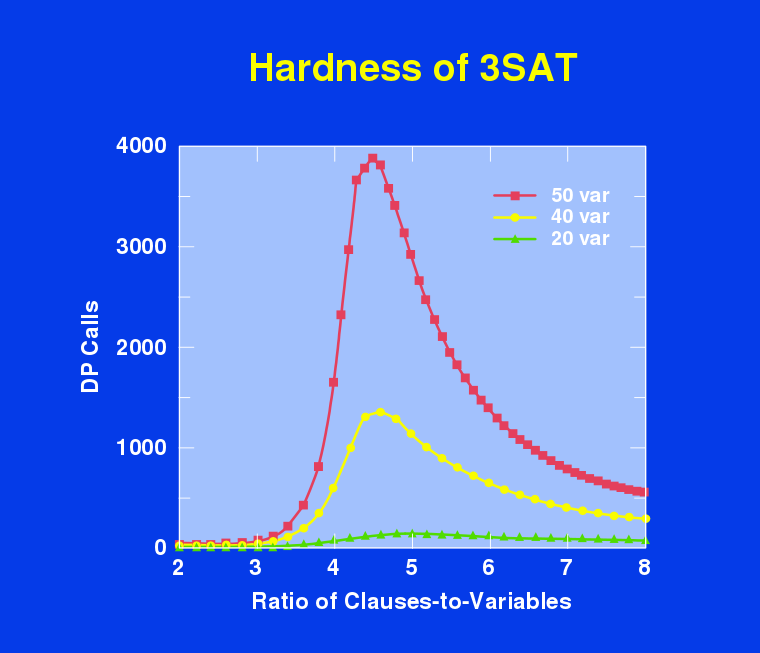
\includegraphics[width=\textwidth]{att.png}
	\caption{Vliv poměru klauzulí a proměnných na obtížnost instance\cite{selman}}
	\label{fig:att}
\end{figure}

\newpage

\subsection{Zkoumání relativní chyby heuristiky}
\label{sec:rel_error}

\subsubsection{Počáteční nastavení parametrů heuristiky a instancí}

Na začátku testování jsem vyzkoušel několik náhodně generovaných instancí, abych odhadl vhodné počáteční nastavení parametrů. Ukázalo se, že podle očekávání má na kvalitu výsledku největší vliv rychlost ochlazování. Počáteční parametry heuristiky jsem tedy zvolil takto:

\begin{table}[h!]
	\centering
	\begin{tabular}{| l | c | }
	\hline
	Počáteční teplota & 80  \\ \hline
	Rychlost ochlazování & 0.999  \\ \hline
        Bod zamrznutí & 0.01  \\
	\hline
	\end{tabular}
	\caption{Počáteční nastavení heuristiky}
	\label{tab:params1}
\end{table}

Pro tyto parametry se ukázalo, že již v instancích s poměrem $ r = 3.\overline{18}$ má heuristika problém nalézt alespoň nějaké řešení. Zvolil jsem tedy následující parametry instancí:

\bgroup
\def\arraystretch{1.2}
\begin{table}[h!]
	\centering
	\begin{tabular}{| l | c | }
	\hline
	Počet proměnných $n$ & 18  \\ \hline
	Počet klauzulí $k$ & 36, 40, 44, 48  \\ \hline
	Poměr $r = k/n$ & 2, $2.\overline{22}$, $2.\overline{44}$, $2.\overline{66}$\\
	\hline
	\end{tabular}
	\caption{Počáteční nastavení parametrů instancí}
	\label{tab:params2}
\end{table}
\egroup

\subsubsection{Měření relativní chyby}
\label{sec:rel_e_measure}

Nyní tedy budeme zkoumat, jak se bude vyvýjet relativní chyba heuristiky v závisloti na zvolených parametrech. Nejprve prozkoumáme vliv rychlosti ochlazování při počítání instancí s parametry popsanými v tabulce \ref{tab:params2}. 

Průměrnou chybu budeme počítat z 50 náhodně vygenerovaných instancí s těmito parametry. Tím by se měl omezit vliv náhodné složky algoritmu.

\begin{figure}[h!]
	\centering
	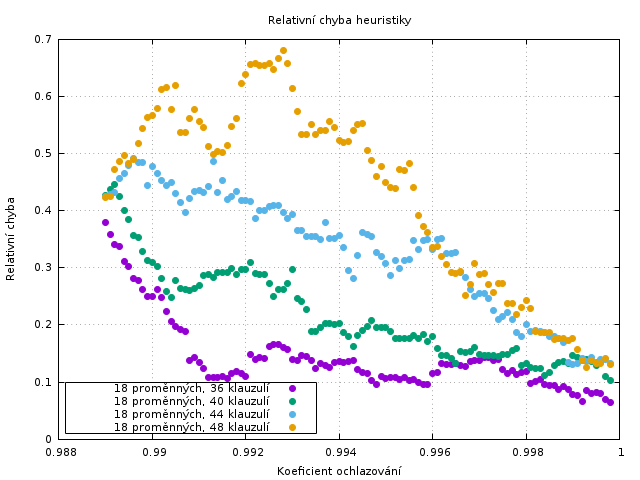
\includegraphics[width=\textwidth]{../grafy/18_40_cooling_e.png}
	\caption{Vliv koeficentu ochlazování na relativní chybu u instancí s $n=18$ a $k=40$}
	\label{fig:18_40_cooling_e}
\end{figure}

Podle očekávání tedy relativní chyba klesá se zvyšujícím se koeficentem ochlazování, což můžeme pozorovat na grafu \ref{fig:18_40_cooling_e}. Můžeme také vidět, že snížení poměru klauzulí k proměnným přineslo předpokládané zlepšení  v chybě heuristiky. Chybu vznikající rostoucím poměrem se do jisté míry daří potlačit pomalejším ochlazováním, ovšem za cenu větší časové náročnosti.

Doba výpočtu naopak s klesající rychlostí ochlazování roste (graf \ref{fig:18_40_cooling_t}), stejně jako u problému batohu. Poměr klauzulí a proměnných dobu běhu nijak neovlivnil. Výpočet cenové funkce je sice datově závislý i na počtu klauzulí, ovšem pouze lineárně, a tak je tato závislost utlumena. 

\begin{figure}[h!]
	\centering
	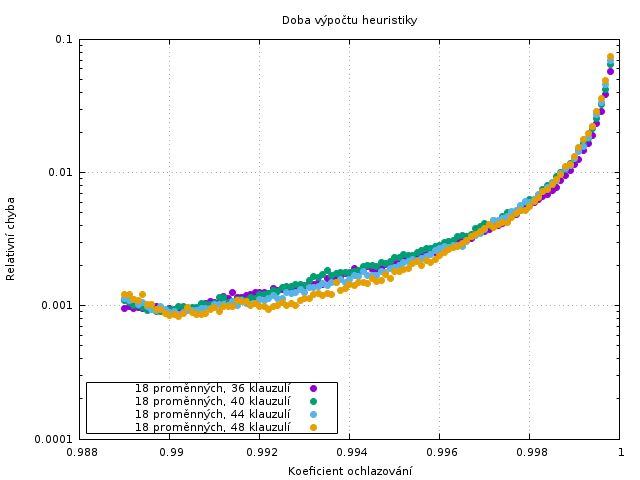
\includegraphics[width=\textwidth]{../grafy/18_40_cooling_t.png}
	\caption{Vliv koeficentu ochlazování na dobu výpočtu u instancí s $n=18$ a $k=40$}
	\label{fig:18_40_cooling_t}
\end{figure}

\subsection{Zkoumání vývoje kvality řešení na větších instancích}

V sekci \ref{sec:rel_error} jsme tedy prozkoumali, jak bude algoritmus reagovat na změnu rychlosti ochlazování a poměru klauzulí k proměnným při počítání malých instancí. Díky malému počtu proměnných jsme mohli najít také optimální řešení a spočítat relativní chybu.

V této sekci budeme zkoumat, jak se algoritmus chová při počítání větších instancí. Vzhledem k tomu, že neznáme optimální řešení nás bude zajímat vývoj kvality nalezeného řešení při zvyšování koeficientu ochlazování a poměru klauzulí k proměnným.

Větší instance jsou zajímavější také z toho důvodu, že vliv poměru klauzulí a proměnných výrazně stoupá (jak je vidět na obrázku \ref{fig:att}). Budeme se tedy snažit volit takový poměr, abychom nalezli alespoň nějaké řešení.

\subsubsection{Počáteční nastavení parametrů heuristiky a instancí}

Vzhledem k tomu, že v tomto případě nás bude zajímat vývoj ceny nalezeného řešení při změně parametrů, nebudeme generovat více instancí, ale v jeden okamžik budeme zkoumat pouze jednu instanci.

Abychom snížili vliv náhodných jevů, budeme výsledky každé instance a každého nastavení průměrovat z deseti běhů algoritmu.

Nejprve jsem se rozhodl otestovat instanci s $n = 50$ a $k = 60$ (tedy $r= 1.2$), se stejným počátečním nastavením heuristiky jako je v tabulce \ref{tab:params1}. 

\subsubsection{Měření vývoje kvality řešení}
\label{sec:measure_q}

Ukázalo se, že i při tomto nízkém poměru (1.2) má v některých případech algoritmus potíže nalézt alespoň nějaké řešení, jak je vidět na grafu \ref{fig:50_60_cooling_v}.

Také průměrná kvalita nalezených řešení značne kolísá kvůli většímu poměru nulových řešení v každém z deseti běhů algoritmu.

\begin{figure}[h!]
	\centering
	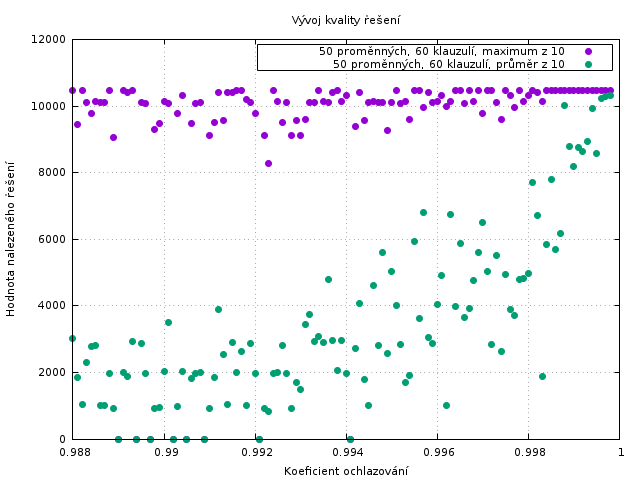
\includegraphics[width=\textwidth]{../grafy/50_60_cooling_v.png}
	\caption{Vývoj kvality řešení při snižování koeficientu ochlazování u instancí s $n=50$ a $k=60$}
	\label{fig:50_60_cooling_v}
\end{figure}

Dále jsem tedy zvýšil zkoumaný koeficient ochlazování (graf \ref{fig:50_60_cooling2_v}). Při tomto pokusu se již heuristice dařilo nalézt nějaké řešení časteji a průměrná kvalita řešení tedy stoupla. Hodnota nejlepšího nalezeného však byla stejná jako v předchozím pokusu.

Zde by tedy bylo možná výhodnější zvolit nižší koeficient ochlazování a provést více běhů algoritmu, neboť zvýšením koeficientu vzrostla pouze frekvence nacházení řešení, ale ne kvalita nejlepšího nalezeného řešení.

\begin{figure}[h!]
	\centering
	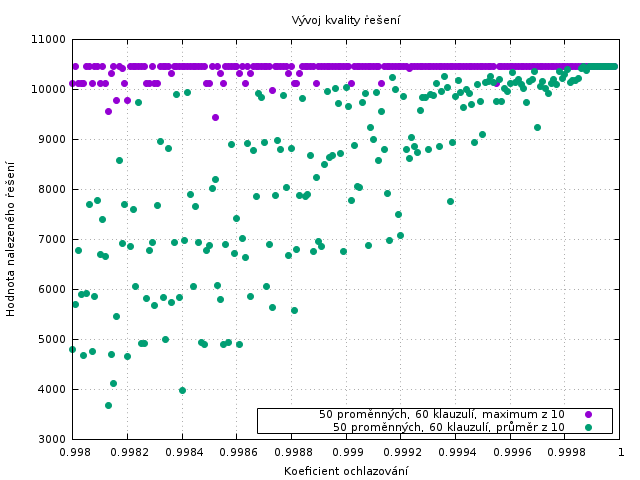
\includegraphics[width=\textwidth]{../grafy/50_60_cooling2_v.png}
	\caption{Vývoj kvality řešení při snižování koeficientu ochlazování u instancí s $n=50$ a $k=60$, (vyšší koeficient)}
	\label{fig:50_60_cooling2_v}
\end{figure}

Každopádně se ukázalo, že vliv poměru klauzulí a proměnných zde působí mnohem silněji než u malých instancí, a je proto potřeba brát v úvahu nejen tento poměr, ale i velikost instance ke které ho vztahujeme.

V dalším pokusu jsem tedy zachoval poměr $k/n = 1.2$, ale snížil počet proměnných na 40. Na grafu \ref{fig:40_48_cooling2_v} je vidět, že v tomto případě se již dařilo algoritmu najít řešení pravidelně, rozptyl v kvalitě řešení je též nižší. To je pravděpodobně opět dáno nižším počtem nulových řešení.

Celkově vývoj kvality nalezeného řešení při pokusech zobrazených na grafech \ref{fig:50_60_cooling_v}, \ref{fig:50_60_cooling2_v} a \ref{fig:40_48_cooling2_v} odpovídal vývoji zobrazeném na grafu \ref{fig:18_40_cooling_e} v sekci \ref{sec:rel_e_measure}. Opět se tedy ukázalo, že nepříznivý poměr klauzulí a proměnných můžeme částečně kompenzovat pomalejším ochlazováním, ovšem za cenu delší doby výpočtu.

\begin{figure}[h!]
	\centering
	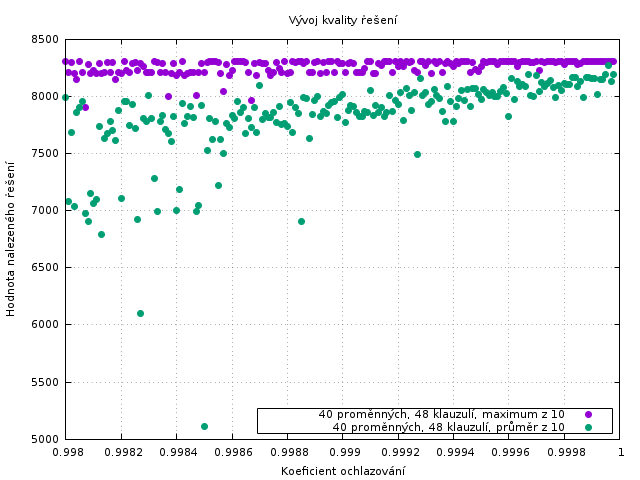
\includegraphics[width=\textwidth]{../grafy/40_48_cooling2_v.png}
	\caption{Vývoj kvality řešení při snižování koeficientu ochlazování u instancí s $n=40$ a $k=48$, (vyšší koeficient)}
	\label{fig:40_48_cooling2_v}
\end{figure}

\subsubsection{Úspěšnost nalezení řešení}

Nakonec jsem zkoumal úspěšnost nalezení alespoň nějakého řešení při rostoucím poměru klauzulí a proměnných $r$. V tomto pokusu jsme zaznamenával počet nenulových řešení z 30 běhů algoritmu na náhodně generovaných instancích s $r$ rostoucím od 1 do 3.

Jak je vidět na grafu \ref{fig:40_success}, úspěšnost rychle klesá k nule pro $r > 2$, a to i při poměrně vysokém koeficientu ochlazování (0.9999). Dále můžeme pozorovat, že mezi instancemi s 50 a 40 proměnnými není výrazný rozdíl v úspěšnosti, dá se ovšem předpokládat snížení průměrné kvality řešení, jak bylo naměřeno v sekci \ref{sec:measure_q}

\begin{figure}[h!]
	\centering
	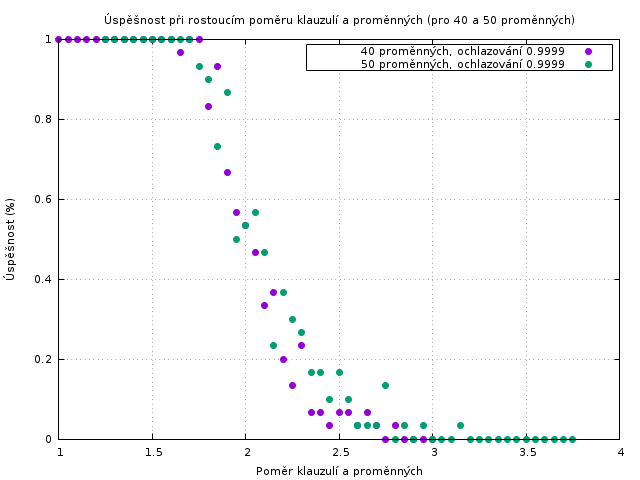
\includegraphics[width=\textwidth]{../grafy/40_success.png}
	\caption{Úspěšnost nalezení řešení při rostoucím poměru klauzulí a proměnných, pro $n = 40$ a $n = 50$}
	\label{fig:40_success}
\end{figure}

\section{Závěr}

V této úloze jsem implementoval algoritmus simulovaného ochlazování řešící 3SAT a otestoval jeho chování na náhodně generovaných instancích.

Ukázalo se, že při vhodném nastavení parametrů se poměrně úspěšně daří řešit instance s poměrem klauzulí a proměnných menším než 2. Rostoucí poměr nepříznivě ovlivňuje kvalitu řešení a při překročení hranice 2.5 se již algoritmu nedaří nalézt žádné řešení splňující zadanou formuli.

Nastavení parametrů heuristiky ovlivňuje míru prohledání stavového prostoru úlohy, a tedy podle očekávání i dobu běhu. Je tedy nutné najít kompromis mezi kvalitou řešení a časovou náročností.

Bohužel úspěšnost nacházení řešení klesá k nule mnohem dřív než je očekávaný mezní poměr 4.3\cite{selman}. Bylo by tedy dále vhodné prozkoumat možná vylepšení implementovaného algoritmu, jako například předzpracování vstupních dat pro volbu lepšího počátečního stavu.

\subsection{Vygenerované instance}

K úloze přikládám instance použité k měření (složka \verb|data|). Soubory s instancemi obsahují popis instance (počet klauzulí, proměnných, váhy a jednotlivé klauzule), a také nejlepší nalezené řešení spolu s parametry při kterých bylo nalezeno.

Malé instance (složka \verb|data/small|) obsahují navíc i optimální řešení nalezené exaktním algoritmem a relativní chybu heuristiky.

\bibliographystyle{csn690}
\bibliography{mybibliographyfile}

\end{document}
